

\chapter{Phylogenetic and functional dissimilarity does not increase during temporal heathland succession} 
\chaptermark{Phylogenetic and functional dissimilarity during succession}

\graphicspath{{Chapter4/Figs}}

\begin{center}

{\large Andrew D. Letten, David A. Keith and Mark G. Tozer}

\small{\textit{\textbf{Proceedings of the Royal Society B}} \textbf{(2014), 281, 20142102}}
\url{http://dx.doi.org/10.1098/rspb.2014.2102}

\vspace{1in}

\includegraphics[width=0.15\linewidth]{Chapter4/Figs/flame2}

\vfill
This study was conceived by ADL with input from DAK. DAK and MGT provided floristic plot data. ADL compiled plant trait data, assembled phylogeny, conducted analyses and wrote the manuscript, with contributions from DAK \& MGT. 

\end{center}

\newpage
\section{Summary}

Succession has been a focal point of ecological research for over a century, but thus far has been poorly explored through the lens of modern phylogenetic and trait-based approaches to community assembly. The vast majority of studies conducted to date have comprised static analyses where communities are observed at a single snapshot in time. Long-term datasets present a vantage point to compare established and emerging theoretical predictions on the phylogenetic and functional trajectory of communities through succession. We investigated within, and between, community measures of phylogenetic and functional diversity in a fire-prone heathland along a 21-year time-series. Contrary to widely-held expectations that increased competition through succession should inhibit the coexistence of species with high niche overlap, plots became more phylogenetically and functionally clustered with time since fire. There were significant directional shifts in individual traits through time indicating deterministic successional processes associated with changing abiotic and/or biotic conditions. However, relative to the observed temporal rate of taxonomic turnover, both phylogenetic and functional turnover were comparatively low, suggesting a degree of functional redundancy amongst close relatives. These results contribute to an emerging body of evidence indicating that limits to the similarity of coexisting species are rarely observed at fine spatial scales.

\newpage
\section{Introduction}

Given limited scope for experimental manipulation in natural systems, a common approach in community ecology is to infer the mechanisms structuring communities from the distribution of their component species and traits. Inferring processes from patterns is of course non-trivial, relying as it necessarily does on a raft of assumptions about how the components of communities (i.e. species) respond to each other and their environment. This \textit{modus operandi} is nowhere more apparent than in the phylogenetic and trait-based analyses of community assembly that have proliferated over the last 10-15 years \citep[e.g.][]{Webb2000, Cornwell2009, Kraft2010}. To date, the vast majority of phylogenetic and trait-based studies of community assembly have comprised `static' analyses where assembly processes are inferred from patterns observed at a single snapshot in time \citep[as reviewed in][]{Swenson2013, Gotzenberger2012}. By necessity, static studies of this kind either ignore the dynamic properties of communities, treat community assembly as a one-off event, or at best assume that observed patterns are representative of prevailing processes. While this assumption may hold in some late successional systems, in dynamic or frequently disturbed systems, the processes that govern community structure may fluctuate considerably over time.

Disentangling sequential assembly processes from observed temporal patterns is complicated by competing and/or unresolved theoretical predictions. One oft-repeated axiom of community ecology holds that competition inhibits species with high niche overlap from coexisting, while environmental filtering has the opposite effect of limiting the range of successful ecological strategies at any one location \citep{Weiher1995, Stubbs2004, Purschke2013}. It follows logically that if ecological niches are phylogenetically conserved, these two apparently opposing processes will leave different signatures on the phylogenetic structure of communities; competition will drive phylogenetic divergence, whilst strong environmental filters will lead to communities consisting largely of close relatives \citep{Webb2000, Webb2002}. Coupling this framework with classical successional theory \citep{Clements1916, Connell1977, Walker1987, Wilson1999}, we might anticipate communities will transition from exhibiting functional and phylogenetic convergence early in succession to becoming increasingly functionally and phylogenetically dispersed as competition increases in relative importance. However, even when niches are phylogenetically conserved, it has recently been argued that this dichotomous framework makes untenable assumptions about the relative importance of niche differences and fitness differences in determining the outcome of community assembly \citep{Chesson2000, Mayfield2010}. As recognised by \citet{Mayfield2010}, when differences in competitive ability exceed niche differences for a large proportion of the species pool, competition may exclude all but the most effective resource competitors. From this alternative perspective, we might predict phylogenetic and functional convergence, rather than divergence, if competition increases through succession. Evidence that competition may indeed drive phylogenetic convergence has recently begun to emerge from a variety of systems and taxa \citep{Kunstler2012, Bennett2013, Price2013, Narwani2013}.

Given the paucity of suitable long-term datasets, most phylogenetic and trait-based research on the effects of disturbance and/or succession on community structure has been limited to static comparisons of relatedness and functional similarity in disturbed versus non-disturbed communities \citep{VERDU2007, Knapp2008, Dinnage2009, Helmus2010}, or across different successional states in a chronosequence (i.e. a space-for-time substitution) \citep{Verdu2009, Letcher2010, Kunstler2012, Purschke2013}. With a few notable exceptions \citep{Verdu2009,Kunstler2012}, most studies have reported greater functional and/or phylogenetic dispersion in undisturbed or late successional communities, including along a rare time series \citep{Norden2012}. Nevertheless, given the known dangers of space-for-time substitutions in ecological research \citep{Johnson2008}, additional temporal successional studies are needed to more robustly explore the generality of this pattern.

An important advantage of phylogenetic and functional analyses of temporal datasets is that it enables the compilation of species pools that are a truer representation of potential colonisers. In the past, static studies have been criticised for deriving species pools from regional species-lists which may include numerous taxa that may never colonise a site even in the absence of competitors \citep{Grime2006, DeBello2012}. This coarse approach may potentially bias analyses towards finding phylogenetic or functional convergence resulting from broad-scale environmental filtering \citep{Gotzenberger2012}. An alternative approach is to try to eliminate the effects of large scale filters \textit{a priori} by constraining the species pool to known colonisers of a site \citep{DeBello2012}. This of course is limited by the availability of data collected over a sufficiently long period of time to record not only those species present at any given time but also the aptly-named dark diversity \citep{Partel2011} i.e. species that may only be competitive (and therefore more likely to be detectable) for a brief period during community assembly/succession. Long-term studies, where the presence of species is monitored at intervals at permanent sites, make this achievable.

In this study we investigated temporal trends in the phylogenetic and functional community structure of understorey plants in fire-prone heathland in southeast Australia. Previous work has provided evidence of strong competitive hierarchies related to vertical stature in this system, with overstorey shrubs typically eliminating understorey species through succession post-fire \citep{Keith1994, Tozer2003, KEITH2007}. However, unlike much of the existing literature on phylogenetic and functional community structure through succession in plant communities \citep[e.g.][]{Letcher2010,Norden2012, Kunstler2012, Bhaskar2014}, here we explicitly focus on understorey communities. With access to compositional data collected over more than 20 years through multiple fire events, this study represents one of the most comprehensive assessments of temporal dynamics in both phylogenetic and functional community structure to date. 

Whilst the phylogenetic and functional structure of plant communities may arise through a complex interplay of various evolutionary (e.g. trait evolution and niche conservatism) and ecological processes (e.g. competition, environmental filtering, herbivory etc.), we concentrated on a subset of hypotheses that reflect the competing theories which have received the most attention in the recent literature. Firstly, assuming fire acts as a filter on the species pool we hypothesised that plots would exhibit functional clustering immediately following fire, and correspondingly also exhibit phylogenetic clustering if the traits mediating early dominance are conserved. Alternatively, if key assembly traits are not conserved, or if measured functional traits have little bearing on community assembly, then we would expect functional and phylogenetic patterns to be uncorrelated. In addition, we made alternative predictions about the trajectories of communities in the period following fire. If increased competition through succession enforces a limit on the similarity of coexisting species, communities should become increasingly functionally dispersed though time, and therefore also phylogeneticaly dispersed if species function is conserved. Alternatively, if increased competition results in the exclusion of all but the most dominant resource competitors \citep[\textit{sensu}][]{Mayfield2010}, or if assembly is primarily driven by fluctuating environmental processes, functional and phylogenetic clustering should remain static or increase through time.  

Our secondary aim was to infer what processes are likely to be driving any observed trends. To this end, we not only considered within community structure but also trends in community-weighted mean trait values and rates of temporal phylogenetic and functional turnover relative to taxonomic turnover. This provided a means to evaluate the extent to which community assembly through succession is structured by deterministic or stochastic processes \citep[e.g.][]{Swenson2012}. For instance, a deterministic model of community assembly assumes that species turnover through time is non-random with respect to species function, and by inference phylogeny. If biotic and abiotic conditions are relatively constant through time, we would predict less phylogenetic and/or functional turnover relative to the observed rate of taxonomic turnover. Conversely, if conditions fluctuate though time, we would predict greater than expected phylogenetic/functional turnover. Finally, if function and phylogeny have no bearing on community assembly \citep[i.e. a stochastic or neutral model \textit{sensu}][]{Hubbell2001}, we should expect taxonomic turnover to be random with respect to phylogeny and function.

\section{Materials and methods}

\subsection{Study site, sampling and fire history}

The study was conducted in an area of fire-prone coastal heathland in Royal National Park, New South Wales, Australia (centred on 34$^{o}$05'46.00" S 151$^{o}$09'02.73" E). The vegetation in the area is characterised by sclerophyllous plants, with a herbaceous ground layer dominated by species within the Restionaceae, Cyperacece and Poaceae families, and woody overstorey layers dominated by shrubs within the Proteaeceae, Myrtaceae, Ericaceae and Fabaceae.  The vegetation is fire-prone, with the herbaceous component regenerating rapidly and gradually becoming overtopped by shrubs within 5-6 years post fire \citep{KEITH2007}. The soils, which derive from sandstone, tend to be highly infertile, acidic and silaceous. The topography is relatively flat with elevations ranging from 68 to 72 m above sea level.

In 1990, fifty-six permanent 0.25 m$^{2}$ plots were established along eight transects arranged in pairs, with each transect comprising seven plots. Plots in each transect pair are spaced an average of 18 metres apart (min = 5 m, max = 45 m), while plots in different transect pairs are separated by an average distance of 211 metres (min = 104 m; max = 323 m). Henceforth we refer to these two discrete spatial scales as the `plot' scale (\textit{n} = 56) and the `site' scale (\textit{n} = 4). Since 1990, the total abundance (number of stems) of all herbaceous species within each plot has been censused on nine separate occasions (1990-1994, 1999, 2002, 2007 and 2011) \citep{Keith2012}.  A fire in 1988 prior to the first census burnt the entire site, with subsequent fires in 1994 (entire site burnt) and 2001 (14 plots along one transect-pair burnt). The 1994 fire occurred prior to the census of that year. 

\subsection{Species pool and community phylogeny}

A species pool was defined comprising all herbaceous angiosperm species (49 unique taxa) recorded across all 56 plots since monitoring began. A species accumulation curves generated from random permutation of samples indicated adequate sampling of the species pool (Appendix C).Non-angiosperms were excluded because they were at low abundance and are known, due to their early divergence from all other species in the pool, to have a disproportionately large effect on metrics of phylogenetic community structure \citep{Kembel2006}. A community phylogeny (figure.~\ref{phylog}), derived from DNA sequence data for two commonly used plastid gene regions (rbcL and matK), was generated using the programs phyloGenerator \citep{Pearse2013} and BEAST \citep{Drummond2007}. Full phylogeny construction details are provided in Appendix C.

 \begin{figure}[H]
 \centering
 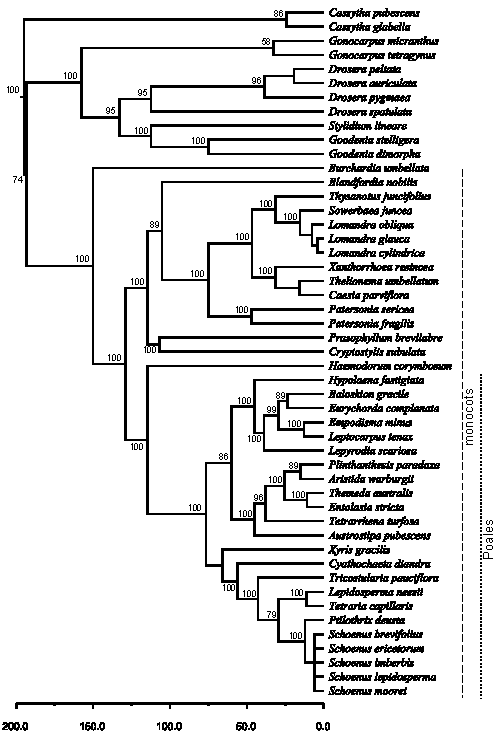
\includegraphics[width=0.9\linewidth]{Chapter4/Figs/phylog_long.pdf}
 \caption{\footnotesize Community phylogeny for all species recorded in plots across the full monitoring period. Vertical dashed/dotted lines denote species belonging to two nested taxonomic groups (monocots and Poales) on which separate analsyes were performed. Node labels denote posterior support values, with unlabelled nodes indicating points where taxa were manually added to the phylogeny post processing. Timescale is in millions of years before present.}
 \label{phylog}
 \end{figure}


\subsection{Functional traits}

All recorded species were scored for seven functional traits related to competitive ability and/or tolerance of disturbance (seed mass, plant height, Raunki\ae r life-form, fire response, fecundity, longevity and seedbank persistence) \citep{Westoby2002, Adler2013a}. All trait data were obtained from existing databases, the primary literature and expert knowledge, with the exception of seed mass which was supplemented with measurements made from herbarium specimens. Seed mass (mg) and plant height (cm) were scored on a continuous scale, while the five remaining traits were coded on an ordinal scale. This included two strictly categorical traits (fire response and life-form) and three implicitly continuous traits (fecundity, longevity and seedbank persistence) that owing to the absence of sufficiently high resolution quantitative data were classified in bins. Fire response was coded with three levels (killed = 1, facultative resprouter = 2, obligate resprouter = 3); life-form with three levels (geophyte = 1, hemicryptophyte = 2, epiphyte = 3); fecundity with four levels (low = 1, low-moderate = 2, moderate = 3, high = 4); longevity with five levels ($<$5 years = 1, 5-10 years = 2,  10-25 years = 3, 25-50 years = 4, $>$50 years = 5); and seedbank persistence with three levels (transient = 1, moderate persistence = 2, persistent = 3). Several commonly measured leaf traits recognised to represent important axes of niche differentiation (e.g. specific leaf area and leaf dry matter content) were not included in the study due to a large proportion of the dominant species lacking true leaves.

In order to assess the correlation between phylogenetic relatedness and functional similarity we tested for significant phylogenetic signal in continuous traits using Blomberg's \textit{K} statistic \citep{Blomberg2003} and in ordinally coded traits using the `fixed tree, character randomly reshuffled' model of \citet{Maddison1991} with ordered costs for character state transitions.

\subsection{Temporal change in phylogenetic and functional community structure}

Phylogenetic community structure within individual plots at each census was evaluated using two commonly used metrics: mean nearest taxon distance (MNTD, mean distance separating each species in each community from it's closest relative), and mean pairwise phylogenetic distance (MPD, mean pairwise distance between all species in each community) \citep{Webb2000, Webb2002}. While these two metrics are typically correlated they provide complementary information, with MNTD being more sensitive to clustering or dispersion near the tips of the phylogeny, and MPD being more sensitive to tree-wide patterns of clustering or dispersion \citep{Kembel2010}. For both MNTD and MPD we used a square-root transformation of phylogenetic distance in order to account for non-linear scaling of phylogenetic relatedness and functional distance \citep{Letten2014}. Standardized effects sizes (SES) for MNTD and MPD were obtained by comparing observed values to those expected under a null model of community assembly. Both observed and null values were quantified using abundance-weighted data. A null model was used that randomly shuffled the names of individuals across the tips of the phylogeny 999 times. This is considered to be the most appropriate null model for temporal analyses \citep{Swenson2012,Norden2012}.    

An identical framework was used to evaluate functional community structure at each census, where the functional analogue of MNTD (F-MNTD) represents the mean distance to each species' nearest neighbour in multi-trait space, and the functional analogue of MPD (F-MPD) represents the mean pairwise distance in multi-trait space between all species in the community. A Gower distance (which allows for range-standardised quantitative and qualitative data) was used to generate the functional distance matrix representing the functional similarity of species in multivariate trait space. 

In order to account for potential sensitivity of community-wide patterns to spatial scale \citep{Swenson2006}, all analyses of individual plots were replicated at a larger spatial scale by summing plot composition within each site (transect-pair, \textit{n} = 4). In addition, whilst we were primarily interested in the trajectory of the full understorey community through time, we replicated all analyses at three nested phylogenetic scales: i) all species; ii) monocots; and iii) Poales (figure.~\ref{phylog}). 

To examine trends in phylogenetic and functional community structure, linear models and linear mixed-models were fit for phylogenetic and functional community structure as a function of time. To account for spatial and temporal non-independence, random effects were fit for transect-pair (random intercept; transect-pairs that didn't burn in 2001 only) and plots (random slope and intercept) at the plot scale, and for transect-pair (random intercept; transect-pairs that didn't burn in 2001 only) at the site scale. Models were fit for either side of the 1994 fire i.e. 1990-1993 and 1994-2011. For the period from 1994-2011, separate models were fit for those plots/transect-pairs that haven't burnt since 1994 (\textit{n} = 42/3) and those that burnt in the 2001 fire (\textit{n} = 14/1). Given that coefficients may be biased for random effects with fewer than five levels, we checked our results against those obtained when using transects (n = 8) as a random effect at the plot scale, and when treating transect as the site grouping at the site scale. All analyses of phylogenetic and functional community structure were performed with the R-package 'picante' \citep{Kembel2010}. An R$^{2}$ summarising the variance in phylogenetic and functional community structure explained by time was calculated using the approach for mixed-effects models provided by \citet{Nakagawa2013} and extended by \citet{Johnson2014}. Finally Welch's t-test was used to determine whether observed differences in the temporal trajectory between sites with different burn frequencies may be attributable to different initial values.

\subsection{Temporal trends in community-weighted mean trait values}

To complement the core analyses, we also investigated temporal trends in community-weighted mean trait values at the plot scale. Community-weighted mean trait values were calculated for each trait in each plot at each time-step by weighting species' trait values by their proportional abundance. For the purposes of obtaining a single value for each trait in each plot, ordinal traits were treated quantitatively. As for measures of phylogenetic and functional community structure, to examine temporal trends, linear models and linear mixed effect models were fit for each community-weighted mean trait value as a function of time. 

\subsection{Temporal phylogenetic and functional beta turnover}

To quantify temporal phylogenetic and functional beta turnover we used between community equivalents of MNTD and MPD which provide a measure of the phylogenetic and functional dissimilarity between pairs of plots sampled over different years \citep{Ricotta2009, Swenson2012}. The formulas for calculating phylogenetic and functional nearest neighbour dissimilarity (\textit{D}$_{nn}$, the beta diversity analogue of MNTD) and pairwise dissimilarity (\textit{D}pw, the beta diversity analogue of MPD) are provided in Appendix C. To determine whether temporal phylogenetic and functional beta diversity was different from that expected given the rate of taxonomic turnover, we compared observed values to those expected under null models. As for MNTD and MPD, null models for \textit{D}$_{nn}$ and \textit{D}$_{pw}$ were generated by randomly shuffling individuals across the tips of the phylogeny or the columns of the functional distance matrix 999 times. Given the large number of possible temporal pairwise comparisons, we only considered the rate of phylogenetic and functional beta turnover of all census points relative to the first census in 1990 and relative to the immediately preceding census point. As for within-community measures, the above analyses were replicated at the two additional phylogenetic scales (monocots and Poales).  

\section{Results}

\subsection{Temporal change in phylogenetic and functional community structure}

Throughout the 20 year survey period, species composition at both spatial scales was consistently phylogenetically clustered relative to the species pool (figure.~\ref{phy_alphadiv}). Clustering was particularly pronounced for MPD with 53\% of plots and 100\% of sites exhibiting signifcant clustering (\textit{SES$_{MPD}$} $<$ -1.96) over the full sampling period. Between 1990 and 1993 there was a weak increase (towards zero from negative) in MNTD at both the plot scale ($R^{2}$ = 0.05, p $<$ 0.001) and the site scale ($R^{2}$ = 0.10, p $<$ 0.05) (figure.~\ref{phy_alphadiv} b \& d), but no significant trend in MPD (figure.~\ref{phy_alphadiv} a \& c). In contrast, following the 1994 fire, both MNTD and MPD exhibited a consistent decreasing trend in those plots (MNTD: $R^{2}$ = 0.10, p $<$ 0.001; MPD:  $R^{2}$ = 0.02, p $<$ 0.05) and sites (MNTD: $R^{2}$ = 0.29, p $<$ 0.005; MPD:  $R^{2}$ = 0.16, p $=$ 0.06) that did not burn again in 2001. The plots and single site that burnt again in 2001 had flatter, non-significant slopes for both MNTD and MPD over the same time interval. 


 \begin{FPfigure}
 %\floatbox[{\capbeside\thisfloatsetup{capbesideposition={right,top},capbesidewidth=7cm}}]{figure}
 {\caption{\footnotesize Phylogenetic and functional community structure through time based on the standardized effect size of: mean pairwise phylogenetic distance (MPD) between all species in each a) plot and c) site; mean phylogenetic distance between nearest taxonomic neighbours (MNTD) in each b) plot and d) site; mean pairwise functional distance (F-MPD) between all species in each e) plot and g) site; mean functional distance between nearest taxonomic neighbours (F-MNTD) in each f) plot and h) site. Trendlines correspond to models of MNTD/MPD vs. time for all plots/sites through the first four years of sampling (solid line); plots/sites that only burnt in 1994 (dashed line) and plots that burnt in 1994 and 2001 (dotted lines). Trend lines shaded black indicate significant slope coefficients at p $<$ 0.05; grey lines indicate insignificant slopes. In a, b, e \& f, boxplot midline corresponds to median value for all 56 plots at each census point; upper and lower hinges give the first and third quartiles; whiskers extend from the hinge to the highest value that is within 1.5 x interquartile range; and data points beyond whiskers are shown as outliers. In c, d, g \& h, open circles correspond to sites that burnt in the 2001 fire; grey-filled circles correspond with sites that did not burn in 2001.}\label{phy_alphadiv}}
 \centering
 {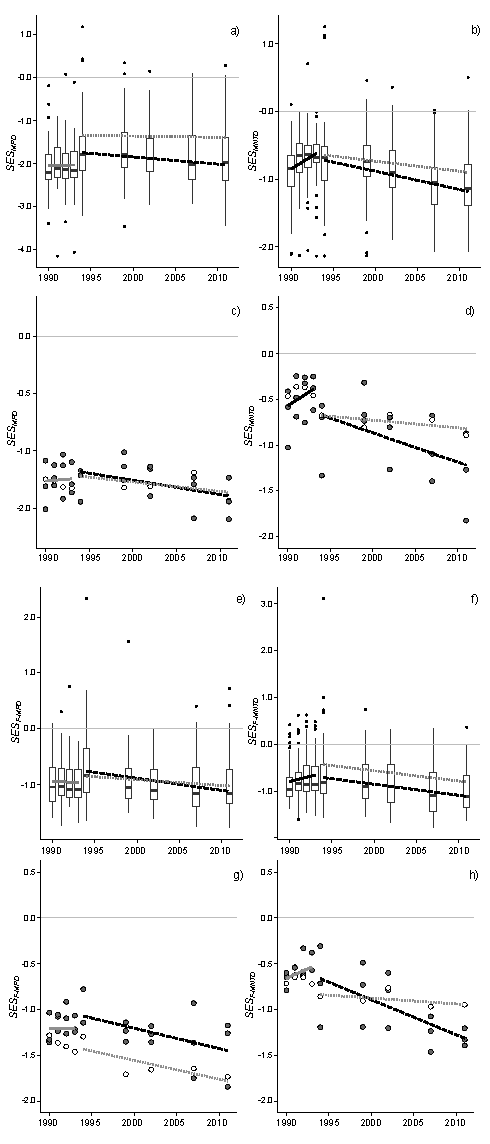
\includegraphics[width=0.65\linewidth]{Chapter4/Figs/eightpanel_resizefont.pdf}}
 \end{FPfigure}

When the species pool was constrained to just monocots or Poales, results were similar to those described for the full species pool with all spatial-phylogenetic scale combinations exhibiting a decreasing trend in MPD and MNTD following the 1994 fire (Appendix C, figure S4.1-S4.2). The only notable difference between the main results and those obtained with reduced species pools was less negative effect sizes in the latter case. This was particularly true for species pools limited to Poales, for which MPD and MNTD was mostly positive, but still low with only MNTD at the plot scale having any ($<$ 1\%) significantly phylogenetically over-dispersed plots over the entire monitoring period. 

All seven measured traits exhibited significant (p $<$ 0.05) phylogenetic signal (Appendix C, table S4.1). In addition, patterns in functional community structure broadly mirrored those observed for phylogenetic community structure. Almost all plots and sites exhibited functional clustering throughout the monitoring period (figure.~\ref{phy_alphadiv} e--h), although notably within the -1.96 threshold for statistical significance. In addition, temporal trends were similar to the phylogenetic analyses, with plots/sites that last burnt in 1994 becoming increasingly functionally clustered through time (plots [F-MNTD: $R^{2}$ = 0.07, p $<$ 0.001; F-MPD:  $R^{2}$ = 0.06, p $<$ 0.001]; sites [F-MNTD: $R^{2}$ = 0.45, p $<$ 0.001; F-MPD:  $R^{2}$ = 0.27, p $<$ 0.05]). As with the phylogenetic analyses, the plots and single site that burnt again in 2001 had flatter, non-significant slopes, although it is important to note that at the site scale statistical power was low given the small number (\textit{n} = 5) of data points. Prior to the 1994 fire, the only significant trend was a very weak increase (towards zero from negative) in F-MNTD at the plot scale ($R^{2}$ = 0.01, p $<$ 0.01]). When the species pool was constrained to just monocots or Poales results were qualitatively identical to the main results (Appendix C, figure S4.3-S4.4), but as for the phylogenetic analyses, effect sizes were reduced.

The observed differences in temporal trajectory cannot be attributed to different initial values given that there was no significant differences at the start of the sampling period between sites with different subsequent burn frequencies (MNTD: \textit{t} = -0.8406, p = 0.4312; MPD: \textit{t} = 0.7769, p = 0.4431; F-MNTD: \textit{t} = 0.7769, p = 0.4431; F-MPD: \textit{t} = 1.3654, p = 0.1812). In addition, coefficients and standard errors were nearly identical when transects was treated as a random effect at the plot scale, or when the site scale was formed by summing abundance across transects rather than transect pairs. Finally, it is worth noting that effect sizes were weaker but remained predominately negative when null randomisations were restricted to those species observed within any given year. 

\subsection{Temporal trends in community-weighted mean trait values}

In common with observed patterns of phylogenetic and functional community structure, temporal trends in mean-trait values tended to differ between plots with different burn frequencies (figure.~\ref{CWM}). Over the four years prior to the 1994 fire, mean-trait values in all plots were comparatively static, with time explaining no more than 3\% of the variation in community weighted mean trait values for any given trait. In contrast, following the 1994 fire, plots within those transects that went unburnt for the remainder of the sampling period exhibited a significant increase in mean seed-weight ($R^{2}$ = 0.07, p $<$ 0.005), longevity ($R^{2}$ = 0.09, p $<$ 0.001) and the proportion of obligate resprouters ($R^{2}$ = 0.16, p $<$ 0.001), and a decrease in fecundity ($R^{2}$ = 0.18, p $<$ 0.001) and the proportion of hemicryptophytes ($R^{2}$ = 0.10, p $<$ 0.001). In contrast, plots that burnt again in 2001 exhibited mostly static mean-trait values, with only a small decrease in fecundity ($R^{2}$ = 0.02, p $<$ 0.001).

\begin{figure}[H]
%\floatbox[{\capbeside\thisfloatsetup{capbesideposition={right,top},capbesidewidth=5cm}}]{figure}
{\caption{\footnotesize Community-weighted mean trait-values through time. Trendlines correspond to models of individual traits vs. time for all plots/sites through the first four years of sampling (solid line); plots/sites that only burnt in 1994 (dashed line) and plots that burnt in 1994 and 2001 (dotted lines). Trend lines shaded black indicate significant slope coefficients at p $<$ 0.05; grey lines indicate insignificant slopes. Boxplot midline corresponds to median value for all 56 plots at each census point; upper and lower hinges give the first and third quartiles; whiskers extend from the hinge to the highest value that is within 1.5 x interquartile range; and data points beyond whiskers are shown as outliers.}\label{CWM}}
{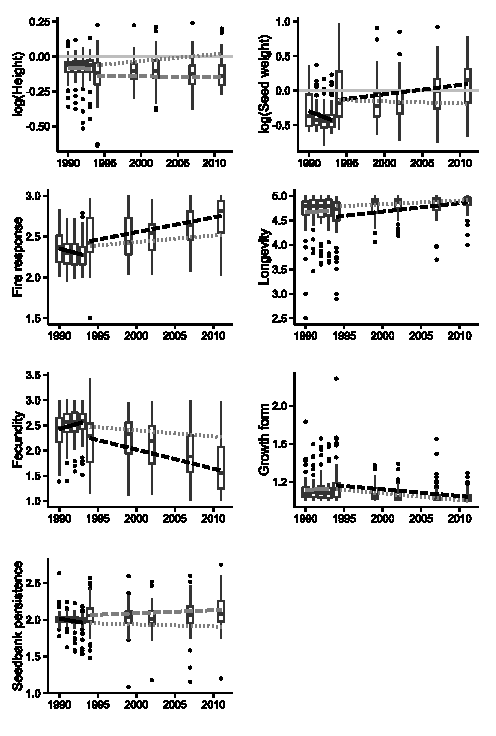
\includegraphics[width=0.8\linewidth]{Chapter4/Figs/CWM.pdf}}
\end{figure}


\subsection{Temporal phylogenetic and functional beta turnover}

Patterns of phylogenetic and functional beta turnover relative to the first census in 1990 were similar to those relative to the immediately preceding census point (for the latter see Appendix C, figure S4.5). Observed temporal phylogenetic turnover was strongly dependent on the metric used and the phylogenetic resolution of the analysis (figure.~\ref{phylo_betadiv}). When evaluated under a nearest-neighbour dissimilarity metric for all species (\textit{D}$_{nn}$), phylogenetic turnover tended to be relatively random with respect to taxonomic turnover, except during early census-point comparisons when some plots showed greater than expected phylogenetic turnover. In contrast, under a pairwise dissimilarity metric (\textit{D}$_{pw}$), temporal phylogenetic turnover was mostly less than that expected given observed taxonomic turnover for all species, but tended to exhibit more random patterns of turnover when the species pool was limited to monocots and in particular to Poales (Appendix C, figure S4.6). Taken together, these results indicate that plot composition through time tended to be constrained from a phylogeny-wide perspective, i.e limited to a small subset of clades (mainly Poales) relative to the community phylogeny. However, within those well represented clades, turnover tended to be either largely random as indicated by (\textit{D}$_{pw}$) for Poales, or occasionally directional as indicated by high values for (\textit{D}$_{nn}$) for the whole phylogeny. This latter inference is based on (\textit{D}$_{nn}$) being more sensitive to turnover near the tips of the phylogeny.   



\begin{figure}[H]
\centering
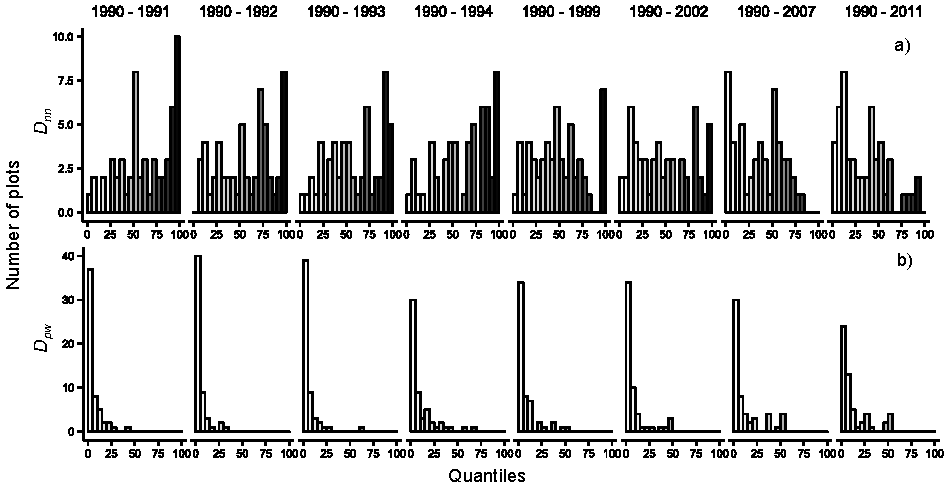
\includegraphics[width=1\linewidth]{Chapter4/Figs/beta_2rows_resize.pdf}
\caption{\footnotesize Temporal phylogenetic beta turnover for all species quantified by a) \textit{D}$_{nn}$, and b) \textit{D}$_{pw}$. Low quantile scores (white) indicate low turnover in phylogenetic composition relative to the observed rate of taxonomic turnover; high quantile scores (black) indicate high turnover in phylogenetic composition relative to the observed rate of taxonomic turnover. Values $<$2.5 or $>$97.5 are significant at the 0.05 level.}
\label{phylo_betadiv}
\end{figure}

For both metrics and all three higher phylogenetic scales, observed temporal functional turnover was less than expected given taxonomic turnover (Appendix C, figure S4.7-S4.9) suggesting that the overall functional composition, as derived from the seven measured traits, was relatively fixed through time. However, as indicated by trends in community-weighted mean trait values and observations of temporal turnover in individual traits, this appeared to be driven by low turnover in several traits, in particular plant height and seedbank persistence. 

\section{Discussion}

A classical axiom of community ecology holds that abiotic processes (e.g. environmental filtering) dominate early in succession, while the relative importance of biotic processes (e.g competition) increases as communities mature \citep{Clements1916, Connell1977, Walker1987, Wilson1999}. Assuming that closely related and functionally similar species compete most intensely, it follows that during succession communities may be expected to transition from those that are dominated by closely related and/or functionally similar taxa to those that comprise more phylogenetically and functionally dispersed assemblages \citep{Purschke2013, Bhaskar2014}. In the present study we found no evidence for an increase in phylogenetic and functional dispersion over 20 years of succession post-fire in a coastal heathland community. Instead, species composition at both the plot scale and the site scale tended on average to become more phylogenetically and functionally clustered over time, except notably in those plots where succession was interrupted by fire. 

These findings contrast with a number of previous studies, where an opposite pattern of increased phylogenetic and/or functional dispersion has been reported in non-disturbed versus disturbed communities \citep{Dinnage2009,Helmus2010}, in late successional stages along chronosequences \citep{Letcher2010, Purschke2013}, and along a rare time series of succession \citep{Norden2012}. However, in several rare exceptions to the rule that echo our own findings, Verdu \textit{et al.} \citep{Verdu2009} found that the competitive exclusion of pioneer species appeared to reduce phylogenetic diversity in the very latter stages of a chronosequence of post-fire succession, while Kunstler \textit{et al.} \citep{Kunstler2012} attributed greater functional and phylogenetic convergence with increasing forest plot age to competition sorting species along a competitive hierarchy in plant height. Most recently, Bhaskar \textit{et al.} \citep{Bhaskar2014} found little evidence for an increase in functional dispersion in secondary tropical forests at various stages post agricultural abandonment. Together with these earlier studies, our results reinforce growing awareness of the complex, and often unpredictable, interaction between community assembly processes and patterns of phylogenetic and functional community structure \citep{Mayfield2010, Kunstler2012, Price2013, Bennett2013}.

While it remains difficult to infer underlying processes from static snapshots of community structure, the observed directional shifts in several community-weighted traits through time are indicative of deterministic turnover in this system. These trends tended to be consistent with predictions based on known relationships between functional traits and life-history strategies \citep{Westoby2002, Adler2013a} i.e. the transition from species with relatively fast life-histories (small seeds, high fecundity and short life-spans) in early succession, to those with slower life histories (large seeds, low fecundity and long life-spans) in late succession (figure.~\ref{CWM}). In particular, the observed increase in community weighted mean seed size, a trait often correlated with shade tolerance \citep{Coomes2003}, is consistent with the replacement of good dispersers and fast germinators/resprouters in the immediate post-fire environment by understorey species with greater shade tolerance as the shrub layer becomes more established. It is also telling that the same traits that exhibited directional shifts in the unburnt plots post 1994, were mostly temporally static in those plots that burnt again in 2001, suggesting that fire prevented the competitive exclusion of early successional species by late successional species. 
 
Mediated by the shrub overstorey, light deprivation to the ground layer may act more like an abiotic stressor external to the system. As such, we might attribute phylogenetic and functional clustering later in succession to a filtering process that is biotic but largely external to the ground layer component of the community. However, even if we treat the effect of shading as an external process, competition for resources in the light deprived understorey is still likely to play a significant role in the assembly process. Indeed, at the local scale of interacting species, relative shade tolerance will translate into fitness differences, whereby the more shade tolerant species are at a competitive advantage. If there is a hierarchy of shade tolerance within the ground layer, competition amongst ground layer species will be expected to drive functional clustering. The notion that competition may drive functional and phylogenetic clustering via hierarchical differences in species' competitive ability was  highlighted by Mayfield and Levine \citep{Mayfield2010}, and has received empirical backing by several recent studies \citep{Kunstler2012, Bennett2013, Narwani2013}. However, to our knowledge this is the first study to present patterns of phylogenetic and functional community structure consistent with this process emerging through a successional time-series.

In spite of the observed directional shifts in community weighted mean-trait values, overall functional and pairwise phylogenetic beta-diversity was comparatively constrained through time. This however was counter-balanced by a relatively high rate of temporal phylogenetic beta-diversity amongst closely related taxa early in succession (\textit{D}$_{nn}$, figure.~\ref{phylo_betadiv}). Together with largely stochastic patterns of turnover amongst the highly represented Poales, a picture emerges of a system in which the dominant species are consistently drawn from a small number of clades within the overall phylogeny. However, within those well represented clades, turnover appears largely stochastic or neutral, with functionally similar close relatives replacing each other through time. This disconnect between results observed at the individual trait level and summary statistics of overall phylogenetic and functional turnover highlights the importance of combined approaches. One explanation is that despite directional shifts in individual traits indicating that the relative fitness of different traits is changing through time, there is still substantial functional redundancy near the tips of the phylogeny, with the fate of individual taxa being relatively stochastic \citep{Rosenfeld2002}.      

Our approach focused specifically on the ground layer within a vertically stratified community, whereas most previous studies of phylogenetic and functional community structure through succession in plant communities have focused on the canopy layer \citep[e.g.][]{Letcher2010,Norden2012} or have been conducted in less vertically stratified communities such as grasslands \citep[e.g.][]{Purschke2013}. Where data are available for both canopy and ground layer components of a community, separate analyses for each strata may be preferable to avoid conflating the relative effects of different assembly processes in each strata. Phylogenetic and functional convergence through succession may be a more general feature of understorey communities than it is of less stratified or canopy `communities' \citep[but see][for an example of convergence amongst canopy species in temperate forests]{Kunstler2012}. Ultimately, more phylogenetic and functional based studies of community assembly through succession in the understorey of vertically stratified communities are needed to verify this hypothesis.

Disentangling the relative contribution of abiotic and biotic processes in driving community assembly through succession remains a major challenge for community ecologists. Contrary to expectations, here we have shown that phylogenetic and functional dispersion is not the only, or necessarily the most likely, outcome of succession. This finding contributes to an emerging body of research re-evaluating the role of limiting functional similarity in determining the outcome of community assembly \citep{Mayfield2010,Kunstler2012, Price2013, Bennett2013}. Efforts to partition out the relative importance of the underlying processes driving functional and phylogenetic convergence through succession in this, and other systems, will be a valuable focus of future work.

\section*{Acknowledgements}

Thanks to Will Pearse for assistance with phyloGenerator, Nate Swenson for providing code for the analysis of phylogenetic and functional beta diversity, and Jodi Price, Will Cornwell and two anonymous reviewers for valuable comments on an earlier draft of this paper.

